\subsection{Simulation Configuration}
\label{sec:eval:cfg}
\begin{figure*}[!t]
\centering
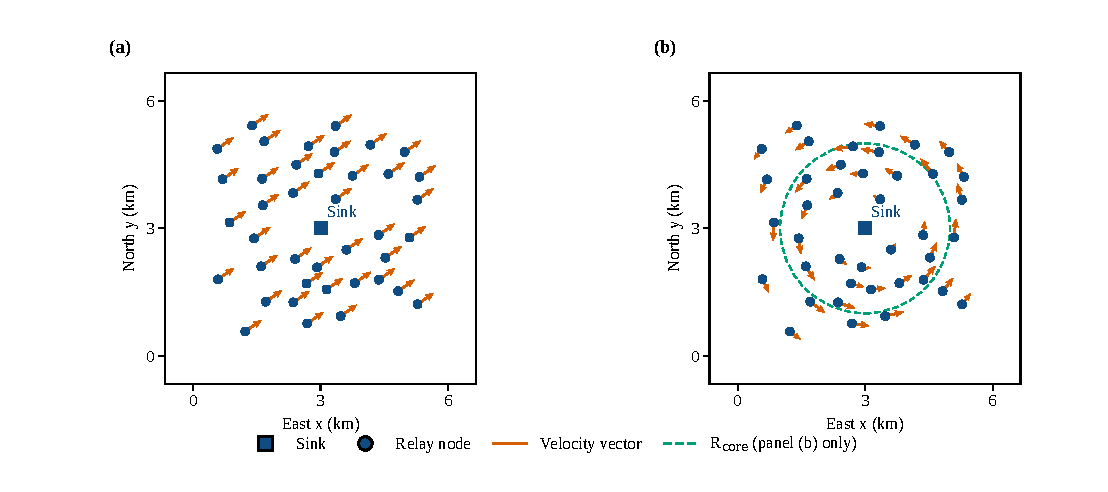
\includegraphics[width=\textwidth]{elqtp_figs/fig2_mobility_fields}
\caption{Velocity fields, $N=40$. (a)~Uniform current, $2\,\mathrm{m/s}$.
(b)~Rankine eddy, $R_{\mathrm{core}}=2000\,\mathrm{m}$.}
\label{fig:mobility_fields}
\end{figure*}

All four protocols share the constants of
Table~\ref{tab:sim_params}: $N=40$ relays in the
$6\,\mathrm{km}\times 6\,\mathrm{km}\times 500\,\mathrm{m}$ column,
January WOA23/GEBCO/Bellhop cell of
Section~\ref{sec:prelim:urick}, $\mathrm{SL}=175\,\mathrm{dB}$,
$R_b=1000\,\mathrm{bit/s}$, $l=400\,\mathrm{bit}$, $M=2$,
$\mathrm{SNR}_{\mathrm{th}}=8.68\,\mathrm{dB}$,
$r_{\mathrm{range}}=5125\,\mathrm{m}$, $E_{\mathrm{ini}}=10000\,\mathrm{J}$,
$\alpha=0.9$, $\gamma=0.8$, and SNR-threshold reception with no
modeled contention.
A node that leaves the area is removed.
Mobile runs use $T_{\mathrm{sim}}=600\,\mathrm{s}$ and
five independent random seeds.
The validated E-LQTP point is the event trigger on and
$\beta_1=\beta_2=0$.
Fixed-Periodic uses the same reward weights and
$T_{\mathrm{ctrl}}=5\,\mathrm{s}$.
That interval is one end-to-end delay of the $v=2\,\mathrm{m/s}$
mesh ($T_{\mathrm{e2e}}\approx 4.4\,\mathrm{s}$; one-hop flight
$\approx 2.0\,\mathrm{s}$ on the Scenario~III $\beta$ sweep).
It is a single, drift-independent budget against which an
event-triggered scheme can be cheaper or more expensive; it is
not claimed to be the optimal periodic timer, and it is the same
class of timer used to rebuild STGR's spatial-temporal graph
\cite{xu2025stgr} and to refresh QTAR and SAQR neighbor state
\cite{nandyala2023qtar,zhang2025saqr}.

% Drop-in for Section IV-A. Values from the campaign in Table I.
% Single-column: short two-column parameter list.

\begin{table}[!t]
\caption{Shared simulation parameters. E-LQTP-only knobs are marked.}
\label{tab:sim_params}
\centering
\scriptsize
\resizebox{\columnwidth}{!}{%
\begin{tabular}{lc}
\hline
Parameter & Value \\
\hline
Volume / $N$ / seeds & $6\,\mathrm{km}\times 6\,\mathrm{km}\times 500\,\mathrm{m}$ / $40$ / five \\
Site / season & $20.125^\circ\mathrm{N}$, $124.125^\circ\mathrm{E}$, January \\
Seafloor / carrier / band & $5524\,\mathrm{m}$ / $24\,\mathrm{kHz}$ / $2\,\mathrm{kHz}$ \\
$\mathrm{SL}$ / $\mathrm{DI}$ / $\mathrm{SNR}_{\mathrm{th}}$ & $175\,\mathrm{dB}$ / $0\,\mathrm{dB}$ / $8.68\,\mathrm{dB}$ \\
$R_b$ / $l$ / $M$ & $1000\,\mathrm{bit/s}$ / $400\,\mathrm{bit}$ / $2$ \\
$r_{\mathrm{range}}$ / $E_{\mathrm{ini}}$ & $5125\,\mathrm{m}$ / $10000\,\mathrm{J}$ \\
Efficiency / $P_{\mathrm{rx}}$ / BER floor & $0.5$ / $0.1\,\mathrm{W}$ / $10^{-9}$ \\
Data interval / $T_{\mathrm{sim}}$ / $dt$ & $30\,\mathrm{s}$ / $600\,\mathrm{s}$ / $1\,\mathrm{s}$ \\
$\alpha$ / $\gamma$ / reception / envelope & $0.9$ / $0.8$ / SNR gate / leave-area nodes removed \\
$\varepsilon_0$ / $s_{\mathrm{cap}}$ / $\lambda$ & $2.0\,\mathrm{dB}$ / $2.0\,\mathrm{dB}$ / $1.0$ \\
$W$ / $W_{\mathrm{mp}}$ / $\rho$ / $T_{\mathrm{ctrl}}$ / $(\beta_1,\beta_2)$ & $5$ / $3$ / $0.6$ / $5\,\mathrm{s}$ / $(0,0)$ \\
\hline
\end{tabular}}
\end{table}


Fig.~\ref{fig:mobility_fields} is the velocity field of the two
mobile scenarios on the same $N=40$ placement and the same fixed
sink.
Panel~(a) is shared current (Scenario~II): every relay has the same
horizontal velocity, so the true AUV--AUV range rate is identically
zero.
The filter does not start from that velocity.
Section~\ref{sec:design:kin} initializes the neighbor-velocity hold
at zero, and the hold takes the true value only after
$\mathrm{Broadcast}_k=1$.
Panel~(b) is the Rankine eddy (Scenario~III): arrow length scales
with local tangential speed, solid-body inside $R_{\mathrm{core}}$
and $1/r$ outside.
The figure's $1/r$ decay is the classical Rankine sketch; the
simulation itself uses the speed cap of \eqref{eq:rankine}.

Three scenarios are reported.
Scenario~I is the stationary identity of
Section~\ref{sec:eval:s1} ($T_{\mathrm{sim}}=1600\,\mathrm{s}$,
EKF not ticked, trigger off) and is a reproduction check, not a
primary mobility result.
Scenario~II sweeps $\|v_{\mathrm{drift}}\|$ at
$0.5$, $1.0$, $2.0$, $3.0$, and $3.5\,\mathrm{m/s}$.
Scenario~III uses $V_{\mathrm{eddy}}=2\,\mathrm{m/s}$ and
$R_{\mathrm{core}}=2000\,\mathrm{m}$.
